Quoting @niemanlab@mastodon.social:
\url{https://mastodon.social/@niemanlab/109836678699676049} \#retoot

\begin{figure}
\centering
\pandocbounded{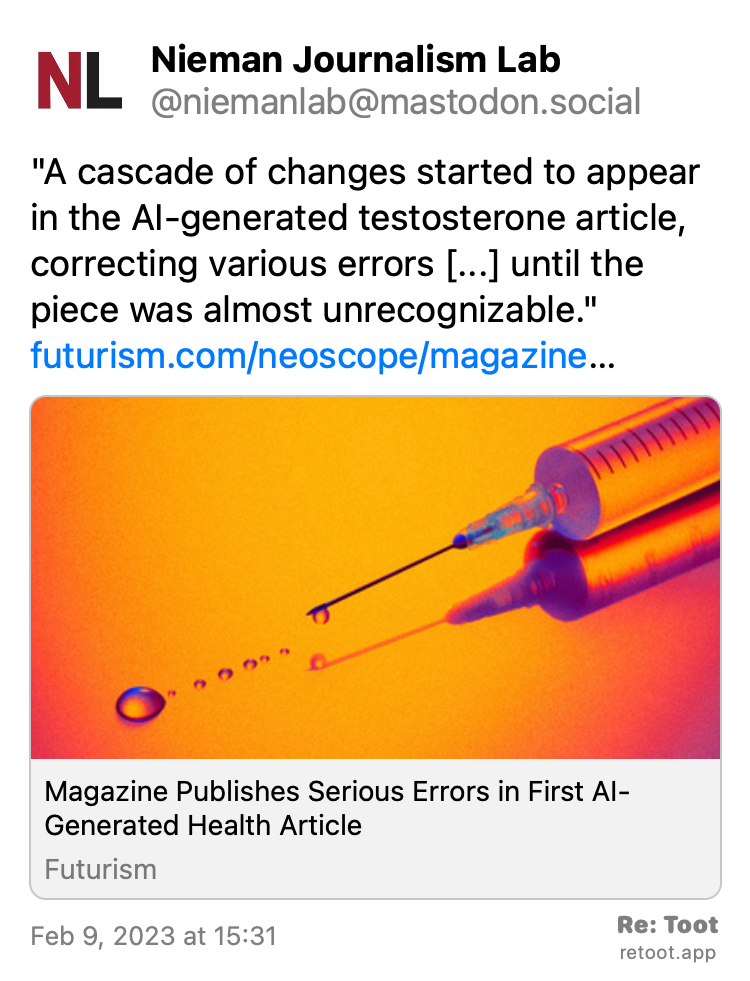
\includegraphics[keepaspectratio]{\%7B\%7Bsite.url\%7D\%7D/img/bad-ai-1.jpg}}
\caption{Post by Nieman Journalism Lab. ``\,``A cascade of changes
started to appear in the AI-generated testosterone article, correcting
various errors {[}\ldots{]} until the piece was almost unrecognizable.''
futurism.com/neoscope/magazine\ldots'' Posted on Feb 9, 2023 at 15:31
https://mastodon.social/@niemanlab/109836678699676049}
\end{figure}

The linked article from Futurism at
\url{https://web.archive.org/web/20230209210750/https://futurism.com/neoscope/magazine-mens-journal-errors-ai-health-article}
is quite the horrifying read. When broken down to its essentials, the
owner of the \emph{Mens Journal} publication tried to substitute AI for
having any writing staff. The results were a very bad mess of incorrect
medical advice.

Other than them getting caught in the end I could see other publications
trying to do this. Humans are expensive and our economy is in a weird
state. We saw \emph{Axios} talking about a crisis facing news
publications in our country
\href{https://web.archive.org/web/20230129153829/https://www.axios.com/2022/07/04/local-newspapers-news-deserts}{in
2022}. Similar discussion was found in \emph{The Guardian}
\href{https://web.archive.org/web/20220625121318/https://www.theguardian.com/media/2020/apr/09/coronavirus-us-newspapers-impact}{in
2020}. Whether we like it or not we're going to see more garbage in the
news ecosystem produced by AI.

Is there a positive way to look at this turn of events? Well, now is
probably a fabulous time to start looking at building out using
\href{https://owncast.online}{owncast} and other tools like possibly
\href{https://www.sourcefabric.org/software/newscoop}{Newscoop}. The
\href{https://www.journalism.cuny.edu/centers/center-community-media/}{Center
for Community Media} led by Jeff Jarvis is probably going to be needed
to help blaze trails in rebuilding this part of the knowledge ecology.
